% Options for packages loaded elsewhere
% Options for packages loaded elsewhere
\PassOptionsToPackage{unicode}{hyperref}
\PassOptionsToPackage{hyphens}{url}
%


\PassOptionsToPackage{table}{xcolor}

\documentclass[
  10pt,
  letterpaper,
]{article}
\usepackage{xcolor}
\usepackage[top=0.85in,left=2.75in,footskip=0.75in]{geometry}
\usepackage{amsmath,amssymb}
\setcounter{secnumdepth}{5}
\usepackage{iftex}
\ifPDFTeX
  \usepackage[T1]{fontenc}
  \usepackage[utf8]{inputenc}
  \usepackage{textcomp} % provide euro and other symbols
\else % if luatex or xetex
  \usepackage{unicode-math} % this also loads fontspec
  \defaultfontfeatures{Scale=MatchLowercase}
  \defaultfontfeatures[\rmfamily]{Ligatures=TeX,Scale=1}
\fi
\usepackage{lmodern}
\ifPDFTeX\else
  % xetex/luatex font selection
\fi
% Use upquote if available, for straight quotes in verbatim environments
\IfFileExists{upquote.sty}{\usepackage{upquote}}{}
\IfFileExists{microtype.sty}{% use microtype if available
  \usepackage[]{microtype}
  \UseMicrotypeSet[protrusion]{basicmath} % disable protrusion for tt fonts
}{}
\makeatletter
\@ifundefined{KOMAClassName}{% if non-KOMA class
  \IfFileExists{parskip.sty}{%
    \usepackage{parskip}
  }{% else
    \setlength{\parindent}{0pt}
    \setlength{\parskip}{6pt plus 2pt minus 1pt}}
}{% if KOMA class
  \KOMAoptions{parskip=half}}
\makeatother


\usepackage{longtable,booktabs,array}
\newcounter{none} % for unnumbered tables
\usepackage{calc} % for calculating minipage widths
% Correct order of tables after \paragraph or \subparagraph
\usepackage{etoolbox}
\makeatletter
\patchcmd\longtable{\par}{\if@noskipsec\mbox{}\fi\par}{}{}
\makeatother
% Allow footnotes in longtable head/foot
\IfFileExists{footnotehyper.sty}{\usepackage{footnotehyper}}{\usepackage{footnote}}
\makesavenoteenv{longtable}
\usepackage{graphicx}
\makeatletter
\newsavebox\pandoc@box
\newcommand*\pandocbounded[1]{% scales image to fit in text height/width
  \sbox\pandoc@box{#1}%
  \Gscale@div\@tempa{\textheight}{\dimexpr\ht\pandoc@box+\dp\pandoc@box\relax}%
  \Gscale@div\@tempb{\linewidth}{\wd\pandoc@box}%
  \ifdim\@tempb\p@<\@tempa\p@\let\@tempa\@tempb\fi% select the smaller of both
  \ifdim\@tempa\p@<\p@\scalebox{\@tempa}{\usebox\pandoc@box}%
  \else\usebox{\pandoc@box}%
  \fi%
}
% Set default figure placement to htbp
\def\fps@figure{htbp}
\makeatother





\setlength{\emergencystretch}{3em} % prevent overfull lines

\providecommand{\tightlist}{%
  \setlength{\itemsep}{0pt}\setlength{\parskip}{0pt}}



 
\usepackage[numbers,square,comma]{natbib}
\bibliographystyle{plos2015}


% Use adjustwidth environment to exceed column width (see example table in text)
\usepackage{changepage}

% marvosym package for additional characters
\usepackage{marvosym}

% cite package, to clean up citations in the main text. Do not remove.
% Using natbib instead
% \usepackage{cite}

% Use nameref to cite supporting information files (see Supporting Information section for more info)
\usepackage{nameref,hyperref}

% line numbers
\usepackage[right]{lineno}

% ligatures disabled
\usepackage{microtype}
\DisableLigatures[f]{encoding = *, family = * }

% create "+" rule type for thick vertical lines
\newcolumntype{+}{!{\vrule width 2pt}}

% create \thickcline for thick horizontal lines of variable length
\newlength\savedwidth
\newcommand\thickcline[1]{%
  \noalign{\global\savedwidth\arrayrulewidth\global\arrayrulewidth 2pt}%
  \cline{#1}%
  \noalign{\vskip\arrayrulewidth}%
  \noalign{\global\arrayrulewidth\savedwidth}%
}

% \thickhline command for thick horizontal lines that span the table
\newcommand\thickhline{\noalign{\global\savedwidth\arrayrulewidth\global\arrayrulewidth 2pt}%
\hline
\noalign{\global\arrayrulewidth\savedwidth}}

% Text layout
\raggedright
\setlength{\parindent}{0.5cm}
\textwidth 5.25in 
\textheight 8.75in

% Bold the 'Figure #' in the caption and separate it from the title/caption with a period
% Captions will be left justified
\usepackage[aboveskip=1pt,labelfont=bf,labelsep=period,justification=raggedright,singlelinecheck=off]{caption}
\renewcommand{\figurename}{Fig}

% Remove brackets from numbering in List of References
\makeatletter
\renewcommand{\@biblabel}[1]{\quad#1.}
\makeatother

% Header and Footer with logo
\usepackage{lastpage,fancyhdr}
\usepackage{epstopdf}
%\pagestyle{myheadings}
\pagestyle{fancy}
\fancyhf{}
%\setlength{\headheight}{27.023pt}
%\lhead{\includegraphics[width=2.0in]{PLOS-submission.eps}}
\rfoot{\thepage/\pageref{LastPage}}
\renewcommand{\headrulewidth}{0pt}
\renewcommand{\footrule}{\hrule height 2pt \vspace{2mm}}
\fancyheadoffset[L]{2.25in}
\fancyfootoffset[L]{2.25in}
\lfoot{\today}
\let\argmax\relax
\DeclareMathOperator*{\argmax}{arg\,max}
\makeatletter
\@ifpackageloaded{caption}{}{\usepackage{caption}}
\AtBeginDocument{%
\ifdefined\contentsname
  \renewcommand*\contentsname{Table of contents}
\else
  \newcommand\contentsname{Table of contents}
\fi
\ifdefined\listfigurename
  \renewcommand*\listfigurename{List of Figures}
\else
  \newcommand\listfigurename{List of Figures}
\fi
\ifdefined\listtablename
  \renewcommand*\listtablename{List of Tables}
\else
  \newcommand\listtablename{List of Tables}
\fi
\ifdefined\figurename
  \renewcommand*\figurename{Figure}
\else
  \newcommand\figurename{Figure}
\fi
\ifdefined\tablename
  \renewcommand*\tablename{Table}
\else
  \newcommand\tablename{Table}
\fi
}
\@ifpackageloaded{float}{}{\usepackage{float}}
\floatstyle{ruled}
\@ifundefined{c@chapter}{\newfloat{codelisting}{h}{lop}}{\newfloat{codelisting}{h}{lop}[chapter]}
\floatname{codelisting}{Listing}
\newcommand*\listoflistings{\listof{codelisting}{List of Listings}}
\makeatother
\makeatletter
\makeatother
\makeatletter
\@ifpackageloaded{caption}{}{\usepackage{caption}}
\@ifpackageloaded{subcaption}{}{\usepackage{subcaption}}
\makeatother
\usepackage{bookmark}
\IfFileExists{xurl.sty}{\usepackage{xurl}}{} % add URL line breaks if available
\urlstyle{same}
\hypersetup{
  pdftitle={Open-Source Python Tools for Annotation and Classification of Marine Acoustic Backscattering},
  pdfauthor={Gaspard Ringuenet; Arnaud Bertrand},
  pdfkeywords={Multi-frequency acoustics, Machine Learning},
  hidelinks,
  pdfcreator={LaTeX via pandoc}}




\begin{document}
\vspace*{0.2in}

% Title must be 250 characters or less.
\begin{flushleft}
{\Large
\textbf\newline{Open-Source Python Tools for Annotation and
Classification of Marine Acoustic
Backscattering} % Please use "sentence case" for title and headings (capitalize only the first word in a title (or heading), the first word in a subtitle (or subheading), and any proper nouns).
}
\newline
\\
% Insert author names, affiliations and corresponding author email (do not include titles, positions, or degrees).
Gaspard Ringuenet\textsuperscript{1*}, Arnaud
Bertrand\textsuperscript{1}
\\
\bigskip
\textbf{1} MARBEC, University of Montpellier, CNRS, Ifremer, IRD, Sète,
France, 
\bigskip

% Insert additional author notes using the symbols described below. Insert symbol callouts after author names as necessary.
% 
% Remove or comment out the author notes below if they aren't used.
%
% Primary Equal Contribution Note

% Additional Equal Contribution Note
% Also use this double-dagger symbol for special authorship notes, such as senior authorship.
%\ddag These authors also contributed equally to this work.

% Current address notes

% Deceased author note

% Group/Consortium Author Note

% Use the asterisk to denote corresponding authorship and provide email address in note below.
* gaspard.ringuenet@umontpellier.fr

\end{flushleft}



\linenumbers

\section{Introduction}\label{introduction}

Active acoustics is nice

\subsection{Key points}\label{key-points}

We propose a set of open-source modular softwares for supervised
echoclassification using traditional ML:

\begin{enumerate}
\def\labelenumi{\arabic{enumi}.}
\tightlist
\item
  A minimalist echogram annotation tool (using a new standard,
  Echoregions)
\item
  A Jupyter notebook workflow class to post-process annotated regions
  and format output as ML-ready dataframe
\item
  The \texttt{escore} Python package containing domain-specific ML tools
  sub-classing scikit-learn estimators and implementing and extending
  the Escore method
\end{enumerate}

As a demonstration we apply the Escore method to the ABRAÇOS campaigns
data.

\pandocbounded{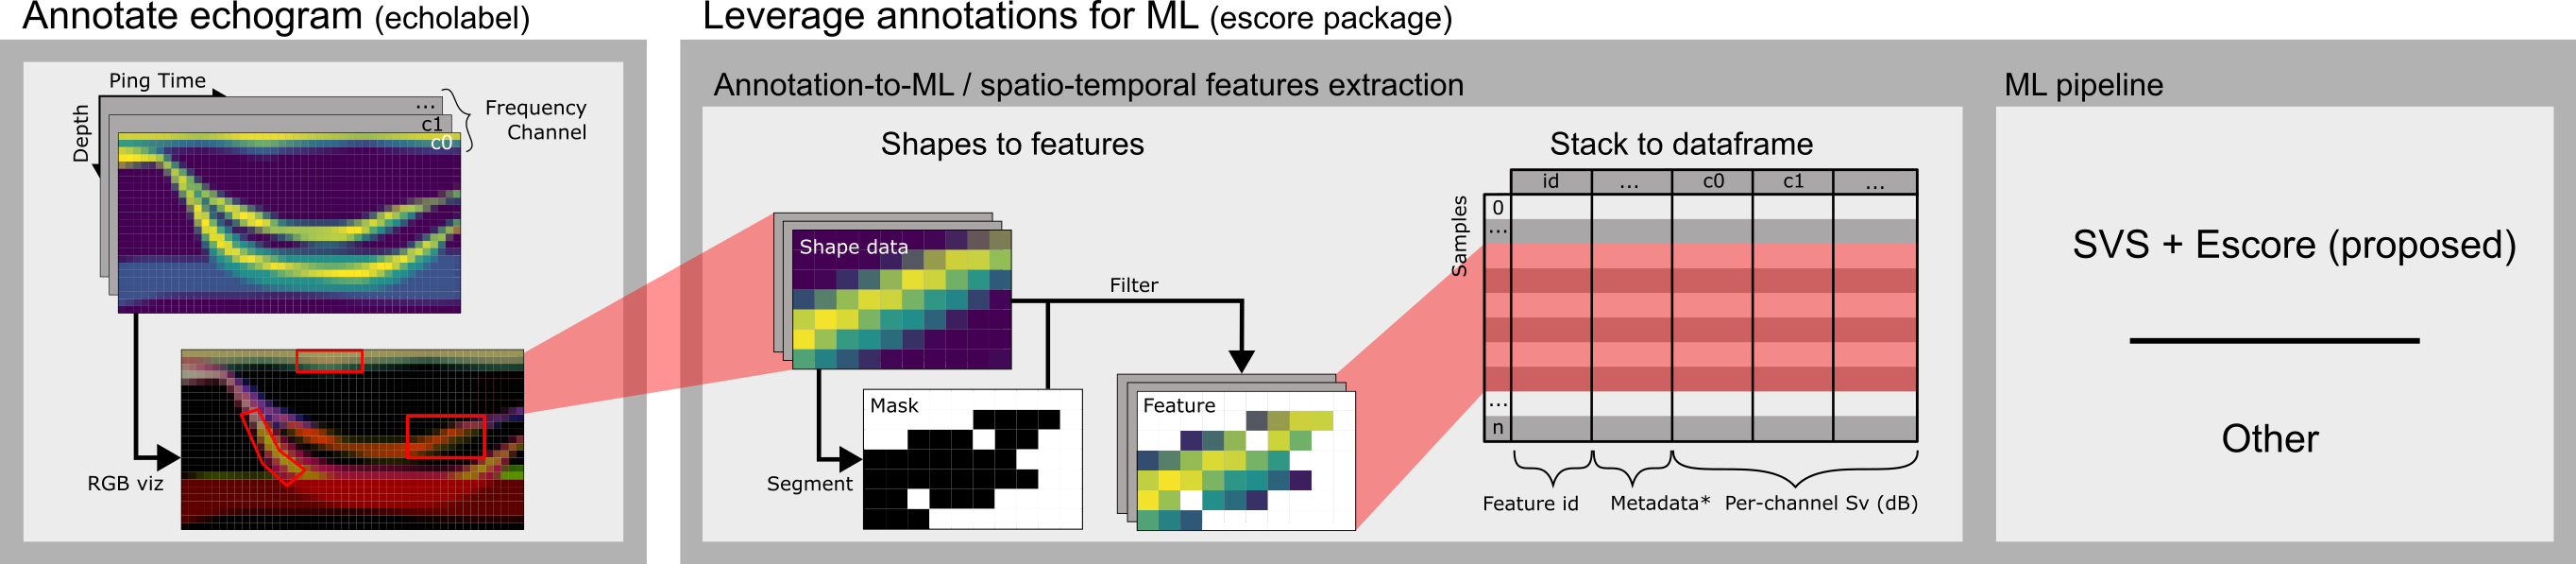
\includegraphics[keepaspectratio]{images/annotation-to-ml-fig.png}}

\section{Tools description}\label{tools-description}

\begin{longtable}[]{@{}ll@{}}
\caption[]{Glossary of terms}\label{tbl-glossary}\tabularnewline
\toprule\noalign{}
Term & Definition \\
\midrule\noalign{}
\endfirsthead
\toprule\noalign{}
Term & Definition \\
\midrule\noalign{}
\endhead
\bottomrule\noalign{}
\endlastfoot
\textbf{Manual echogram annotation concepts} & \\
Region & Echogram region delimited by a 2D polygonal shape. In the
plural, also designates the corresponding Python representation, or
annotation file. \\
Echogram feature & Any spatio-temporal feature visible on the echogram.
\emph{E.g.} shoal, scattering layer, aggregation, internal wave. Such
feature is easily spotted by the operator. Extracting it for analysis or
modeling is crucial. \\
Feature Library & A set of echogram features, potentially including
metadata such as user-defined class name. Feature libraries are used as
training sets for modeling tasks. \\
\textbf{Escore specific terms} & \\
Strong and Variable Scatters (SVS) & Fish-like echoes characterized with
very strong \(S_v\) values, and important variability within the same
aggregation. \\
Region of Interest (ROI) & ``Manually chosen section of the RGB echogram
which contains a specific structure of interest with consistent
frequency responses'' \citep{annasawmy2024}. An ROI is an
Escore-specific \emph{Region}. \\
Echo-type & Underlying echogram feature contained within an ROI,
typically extracted using a KMeans clustering of relative frequeny
response. \\
Echo-class & Grouping of \emph{Echo-types} sharing similar relative
frequency response. In the Escore algorithm, echo-class are create using
a hierarchical clustering of an echo-types library using mean relative
frequency response. \\
\end{longtable}

\subsection{Echolabel: image-based echogram annotation
tool}\label{echolabel-image-based-echogram-annotation-tool}

We propose Echolabel, an open-source minimalist Python application for
interactive echogram annotation. The tool is designed to enable
polygonal shapes annotation without relying on heavy - and often costly
- active acoustics softwares \citep[see][ for existing
softwares]{lee2024a}.

The design is simple: converting acoustic data into echogram images, and
running an image annotation software with a graphical user interface
(GUI) to draw shapes on those images. Echolabel wraps LabelMe\footnote{LabelMe
  runs locally. Its key feature is a GUI built with PyQt5, allowing the
  user to draw shapes (namely polygons and lines) over the images.}
(\url{https://labelme.io/}), is a popular image annotation software
designed to build computer vision datasets, which was inspired by the
Massachusetts Institute of Technology's LabelMe web-based interface
\citep{russell2008} and provides an open-source Python implementation
with added features.

The application is run via a command line interface. Required arguments
are source (acoustic data file(s)) and output (annotation file).
Echogram visualization options can be specified, including mapped
frequency channels and color mapping. Options can be provided as command
line arguments or by editing the user's configuration file, allowing
pre-defined setup.

As input acoustic data, Echolabel expects gridded data with time, depth
and channel dimensions, as well as an acoustic variable (typically
``Sv''). Support is provided by default for the IMOS convention
\citep{kunnath2018} and Echopype products by trying known coordinate
names (e.g.~for time dimension: ``time'' and ``ping\_time''). The former
is a \emph{de facto} standard used by many large-scale databases while
the latter is the new open-source reference software for acoustic data
processing. However, since existing datasets follow varying standards we
chose to let the user specify coordinates and variable names in the
configuration file. One or more NetCDF files may be loaded if
compatible. A Zarr store is also accepted as input.

When launched, the Echolabel reads the source data, chunks it into
fixed-width frames, and saves the frames' metadata. Frames are converted
into images by applying a color mapping. Three channels can be rendered
simultaneously using an RGB mapping \citep{ariza2022}, providing visual
intuition on the organisms' frequency responses. The Labelme graphical
user interface is then launched. As long as the window remains open, the
user can add and edit shapes on the dataset's images. When closing,
shapes are converted to (time, depth) coordinates using cached images
metadata and the annotation file is (over-)written.

For more details, refer to the online documentation
(\url{https://echolabel.readthedocs.io/}).

Converting echograms to images comes at a cost: losing time and depth
label, enforcing a 1:1 aspect ratio for sampled volumes, having no
access to the numeric values of pixels. However, many annotation tasks
can still be performed efficiently (identifying and delineating
aggregations, or finding regions of interest for the Escore algorithm).
Besides, image files are much lighter than original data, and their
rendering is optimized by LabelMe. This enables fast scrolling through
the echogram, and eventually improves user experience and processing
speed. A current limitation, however, is LabelMe's default smoothing
behaviour. This blurs the signal at a small scale when zooming and is
problematic when looking for the edge of an echogram feature. Echolabel
currently deletes shapes that span more than one echogram image. This is
an issue when editing annotation files made with a different software or
image width.

\subsection{Escore: broad-ecosystem semi-supervised thresholding
package}\label{escore-broad-ecosystem-semi-supervised-thresholding-package}

\subsubsection{Echogram feature extraction
utility}\label{echogram-feature-extraction-utility}

Once a set of echogram regions has been defined and stored as an
annotation file, using those within a traditional ML pipeline requires
extracting the samples and assembling them as a tabular dataset with one
row per sample\footnote{This is recommended for
  \href{https://scikit-learn.org/stable/data_interoperability.html}{scikit-learn}
  pipelines at least.}. Additionally, because of high pixel-wise
variability in acoustic response, delineating echogram features with
polygons is often not sufficient to catch the desired signal.
Post-processing of regions, for instance using frequency response
clustering, can be necessary to extract complex objects or reduce signal
variability. Such a treatment requires close supervision by the operator
in order to select meaningful data.

The \texttt{ExtractionWorkflow} class provides a framework and utilities
for the post-processing of region data. Parametrized by an acoustic
dataset\footnote{Would be nice to have: (1) optionally time and depth as
  features (2) simple ``None'' value for when we do not want to segment
  (3) segmenter as a more general callable? (currently limited bc. using
  \texttt{.fit\_predict})} and the corresponding region annotations
(\texttt{Regions2D} object), it allows the user to loop through all
regions, perform segmentation tasks, and save or reject the result.
Built to be used in a Jupyter notebook, the workflow class also enables
rich visualization of input and results during processing. Plots include
echograms and frequency response statistics, and many made interactive
using the hvPlot library.

The core objective of the workflow is selecting a subset of each region.
This is done using a \emph{segmenter}. The segmenter is a classification
function taking the region's channel dimension as features\footnote{Would
  be nice to have: (1) optionally time and depth as features (2) simple
  ``None'' value for when we do not want to segment (3) segmenter as a
  more general callable? (currently limited bc. using
  \texttt{.fit\_predict})}. While we show the use of custom segmenters
such as clustering models in Section~\ref{sec-case-study}, the user is
allowed to set their own depending on their extraction goals.

The workflow object stores the segmentation results and recipes
(segmentation model, selected segment) as files, enabling full
reproducibility of the interactive process. Once the user is satisfied
with the processed regions, all samples can be exported as a dataframe
for further use in ML pipelines.

\subsubsection{SVS algorithm}\label{svs-algorithm}

Algorithm description (Gary Vargas' flow chart) Module features.

\subsubsection{Escore model}\label{escore-model}

The Ellipsoïd score (Escore) method is a dB-differencing method
introduced by \citet{annasawmy2024}. It is a generalization of the
Z-score \citep{derobertis2010} for more than 2 frequencies. The Escore
is adapted to the lack of easily separable aggregation and the sparsity
of trawling coverage by relying on expert RGB composite echogram
scrutinizing rather than ground-truth.

The key idea of the method is analoguous to building an image's
\emph{color palette} by selecting reference areas. Instead of colors,
the Escore model operates on relative frequency responses
(i.e.~\(\Delta \text{MVBS}\)). It lets the user select small regions of
the echogram, named \emph{regions of interest} (ROI), each containing a
structure of interest with homogeneous frequency response. Selected
frequency responses are then extracted, grouped into \emph{echoclasses}
and modeled as Gaussian distribution in \(\Delta \text{MVBS}\) space.
See \citet{annasawmy2024} for a more detailed explanation of the method.
Our implementation incorporates adaptations, mostly related to the
integration within the scikit-learn framework. Some methodological
changes are also applied, mainly to increase interpretability of the
model's output;

In a modular approach, the user is left to complete the ROI selection
step with the echogram annotation software of their choice, as long as
the annotation format can be read as a \texttt{Regions2D} object. The
\texttt{ExtractionWorkflow} can then be used to extract echo-types using
a KMeans clustering of \(\Delta \text{MVBS}\) as segmenter. Following
the Escore nomenclature, the extracted segments are called echo-types.

In a similar manner, grouping can be achieved using the scikit-learn
framework. We only provide simple utility functions to inspect and
evaluate clustering performance. With regards to the model itself, we
propose some changes. To begin with, we dropped step 4, unsure of the
additional benefits compared to applying step 5 to all echoclasses.

We designed a custom scikit-learn estimator called
\texttt{EscoreClassifier}. In a slight change from the original
description, we re-interpreted the Escore model as a combination of
Gaussian distributions in \(\Delta \text{MVBS}\) space, one for each
echo-class. Learning this supervised model comes down to learning the
parameters of those distributions, i.e.~still the echo-classes' means
and covariance matrices. The model can then predict the Mahalanobis
distance of a given point \(x\) to each distribution. That distance can
in turn be used to compute the likelihood of \(\mathbb{P}(x|c)\) for any
echo-class \(c\). This probabilistic formulation adds some
interpretability to an otherwise abstract distance measure. One could
also want to derive the posterior probabilities \(\mathbb{P}(c|x)\), but
this is out of this work's scope.

In addition to learned parameters, our model is also defined by two
hyper parameters corresponding to prediction thresholds. The first one
is equivalent to the original Escore threshold. It defined the minimal
likelihood for prediction. The second one is a quality threshold
controlling the maximum acceptable ratio of likelihoods between the best
and second best class. This avoids predicting at the boundaries between
echo-classes, which might be welcome in some cases.

As a mathematical formulation, we consider a set of echoclasses \(C\),
and we assume that the conditional probability distribution of each
echoclass follows a normal distribution:

\[
\forall c \in C, \mathbb{P}(.|c) \sim \mathcal{N}(\mu_c, \Sigma_c)
\]

Assuming an \(n\)-dimensional \(\Delta \text{MVBS}\) space and
\(x \in \mathbb{R}^n\), the best and second best echoclass predictions
for \(x\) can be defined as:

\[
c_1 = \argmax_c{\mathbb{P}(x|c)}
\]

\[
c_2 = \argmax_{c \neq c_1}{\mathbb{P}(x|c)}
\]

Our model is the prediction function \(f\) such that:

\[
f(x) = \left\{ \begin{array}{ll}
-1 & : \mathbb{P}(x|c_1) < e_{\text{thresh}} \ \cup \ \mathbb{P}(x|c_2) / \mathbb{P}(x|c_1) >  q_{\text{thresh}} \\
c_1 & : else
\end{array} \right.
\]

where \(-1\) is a rejection value returned when the thresholds
constraints are violated.

Integrating into the scikit-learn API brings some notable benefits. In
particular, this unlocks support for cross validation and a wide range
of other machine learning utilities.

\subsubsection{Methodology
recommandations}\label{methodology-recommandations}

\begin{itemize}
\tightlist
\item
  Acoustic community
\item
  Echo-types selection

  \begin{itemize}
  \tightlist
  \item
    Quality is hard to assess
  \item
    R(f) + shape criteria
  \item
    An opinionated process: choices should be made explicit
  \item
    Model validity
  \end{itemize}
\end{itemize}

By design the Escore method is performed in the absence of ground-truth
data. This aspect is a strength in context in which little such data
exists, as it enables \emph{non-arbitrary classification}\footnote{Because
  in many cases classical \(\Delta \text{MVBS}\) clustering methods are.}
of the echoes. However, this also implies less safeguard in case of the
method is poorly executed. In this section, we review the methods
objectives, before diving into methodological recommendations related to
echo-types selection.

\textbf{Acoustic communities}

The goal of the method is to model the relative frequency responses of
the \emph{acoustic communities} present in the data. The term refers to
the ecological definition of a community , that is a collection of
species populations occupying the same space and interacting with one
another \citep{putman1984}. Acoustic communities designates populations
whose co-occurrence is detected by active acoustics systems. The term is
adapted to highly diverse pelagic environments, where chance is high
that a sampled volume contain several backscattering species. Even if a
single organism or species were sampled, the acoustic resolution would
not be sufficient to classify it at the species level
(e.g.~\textasciitilde{} XXX swim bladder-bearing mesopelagic fish
species were caught during the ABRAÇOS I survey).

\emph{How to define an acoustic community in practice?}

\begin{itemize}
\tightlist
\item
  frequency response
\item
  spatio-temporal extent
\item
  frequency of observation
\end{itemize}

\textbf{Training set definition}

The ROI selected during the first step of the Escore method must contain
echo-types representative of the local\footnote{What do we mean by
  local? (That is the question).} acoustic communities.

\emph{What about picking at random?}

\emph{Existing criteria}

The definition proposed by \citet{annasawmy2024} provides a first
selection guideline by specifying two characteristics of the signal
within an ROI: a structure of interest and consistent frequency
responses. Their implementation enforces those assumptions during
echo-types extraction. KMeans clustering of \(\Delta \text{MVBS}\) must
produce a segment:

\begin{enumerate}
\def\labelenumi{\arabic{enumi}.}
\tightlist
\item
  containing the desired spatio-temporal structure, with little
  alteration
\item
  whose relative frequency response is normal for all frequencies (other
  than the reference frequency)
\item
  whose relative frequency standard deviation is small for all
  frequencies (other than the reference frequency)
\end{enumerate}

We find the normality criteria to be too restrictive, in particular when
considering small ROIs, such as the 120 kHz crustacean patches.

We propose to allow selection as long as criteria 1 or criteria 2 are
respected (criteria 3 remains mandatory).

\emph{Recommendations}

In spite of guideline, ROI selection is subjective. Potential ROIs are
numerous and indeterminate. Selecting them is often made using
assumptions on what a ``good signal'' is, and by specifically looking
for suspected acoustic communities.

``Good signal'' heuristics can include:

\begin{enumerate}
\def\labelenumi{\arabic{enumi}.}
\tightlist
\item
  looking for the ``core'' or for ``clean'' frequency response: the
  operator looks for structure that seem to be less diverse in species,
  typically during daytime or during diel vertical migration. A
  potential bias, however, is to look for bright red, green or blue on
  the RGB echogram. Strong frequency response for one channel is not
  necessarily associated to a more ``pure'' sample composition.
\end{enumerate}

We recommend that authors establish a prior typology of echogram
features believed to be associated to specific acoustic communities.
Such typology should be published as part of the results.

\textbf{Model validation}

Visual validation using predicted class masks at the scale of a survey
may be somewhat informative. However, it should be noted that all
relative frequency response clustering techniques tend to result in
``good-looking'' masks when comparing to the RGB echogram, no matter how
arbitrary the boundaries are. This biased is easy to understand, as the
echogram is split according to color\footnote{Could be more precise.
  Typical split depends on G-R and B-R.}.

\textbf{Model validity}

Like any ecological community, and especially pelagic ones, acoustic
communities are defined in space and time. Hence, the validity of an
Escore model is limited to the spatio-temporal range of the modelled
communities.

\begin{itemize}
\tightlist
\item
  Spatial variations?
\item
  Temporal variations: long-term, seasonal and most importantly diel.
\end{itemize}

\section{Case-study: echoclassification in high diversity
context}\label{sec-case-study}

\begin{center}
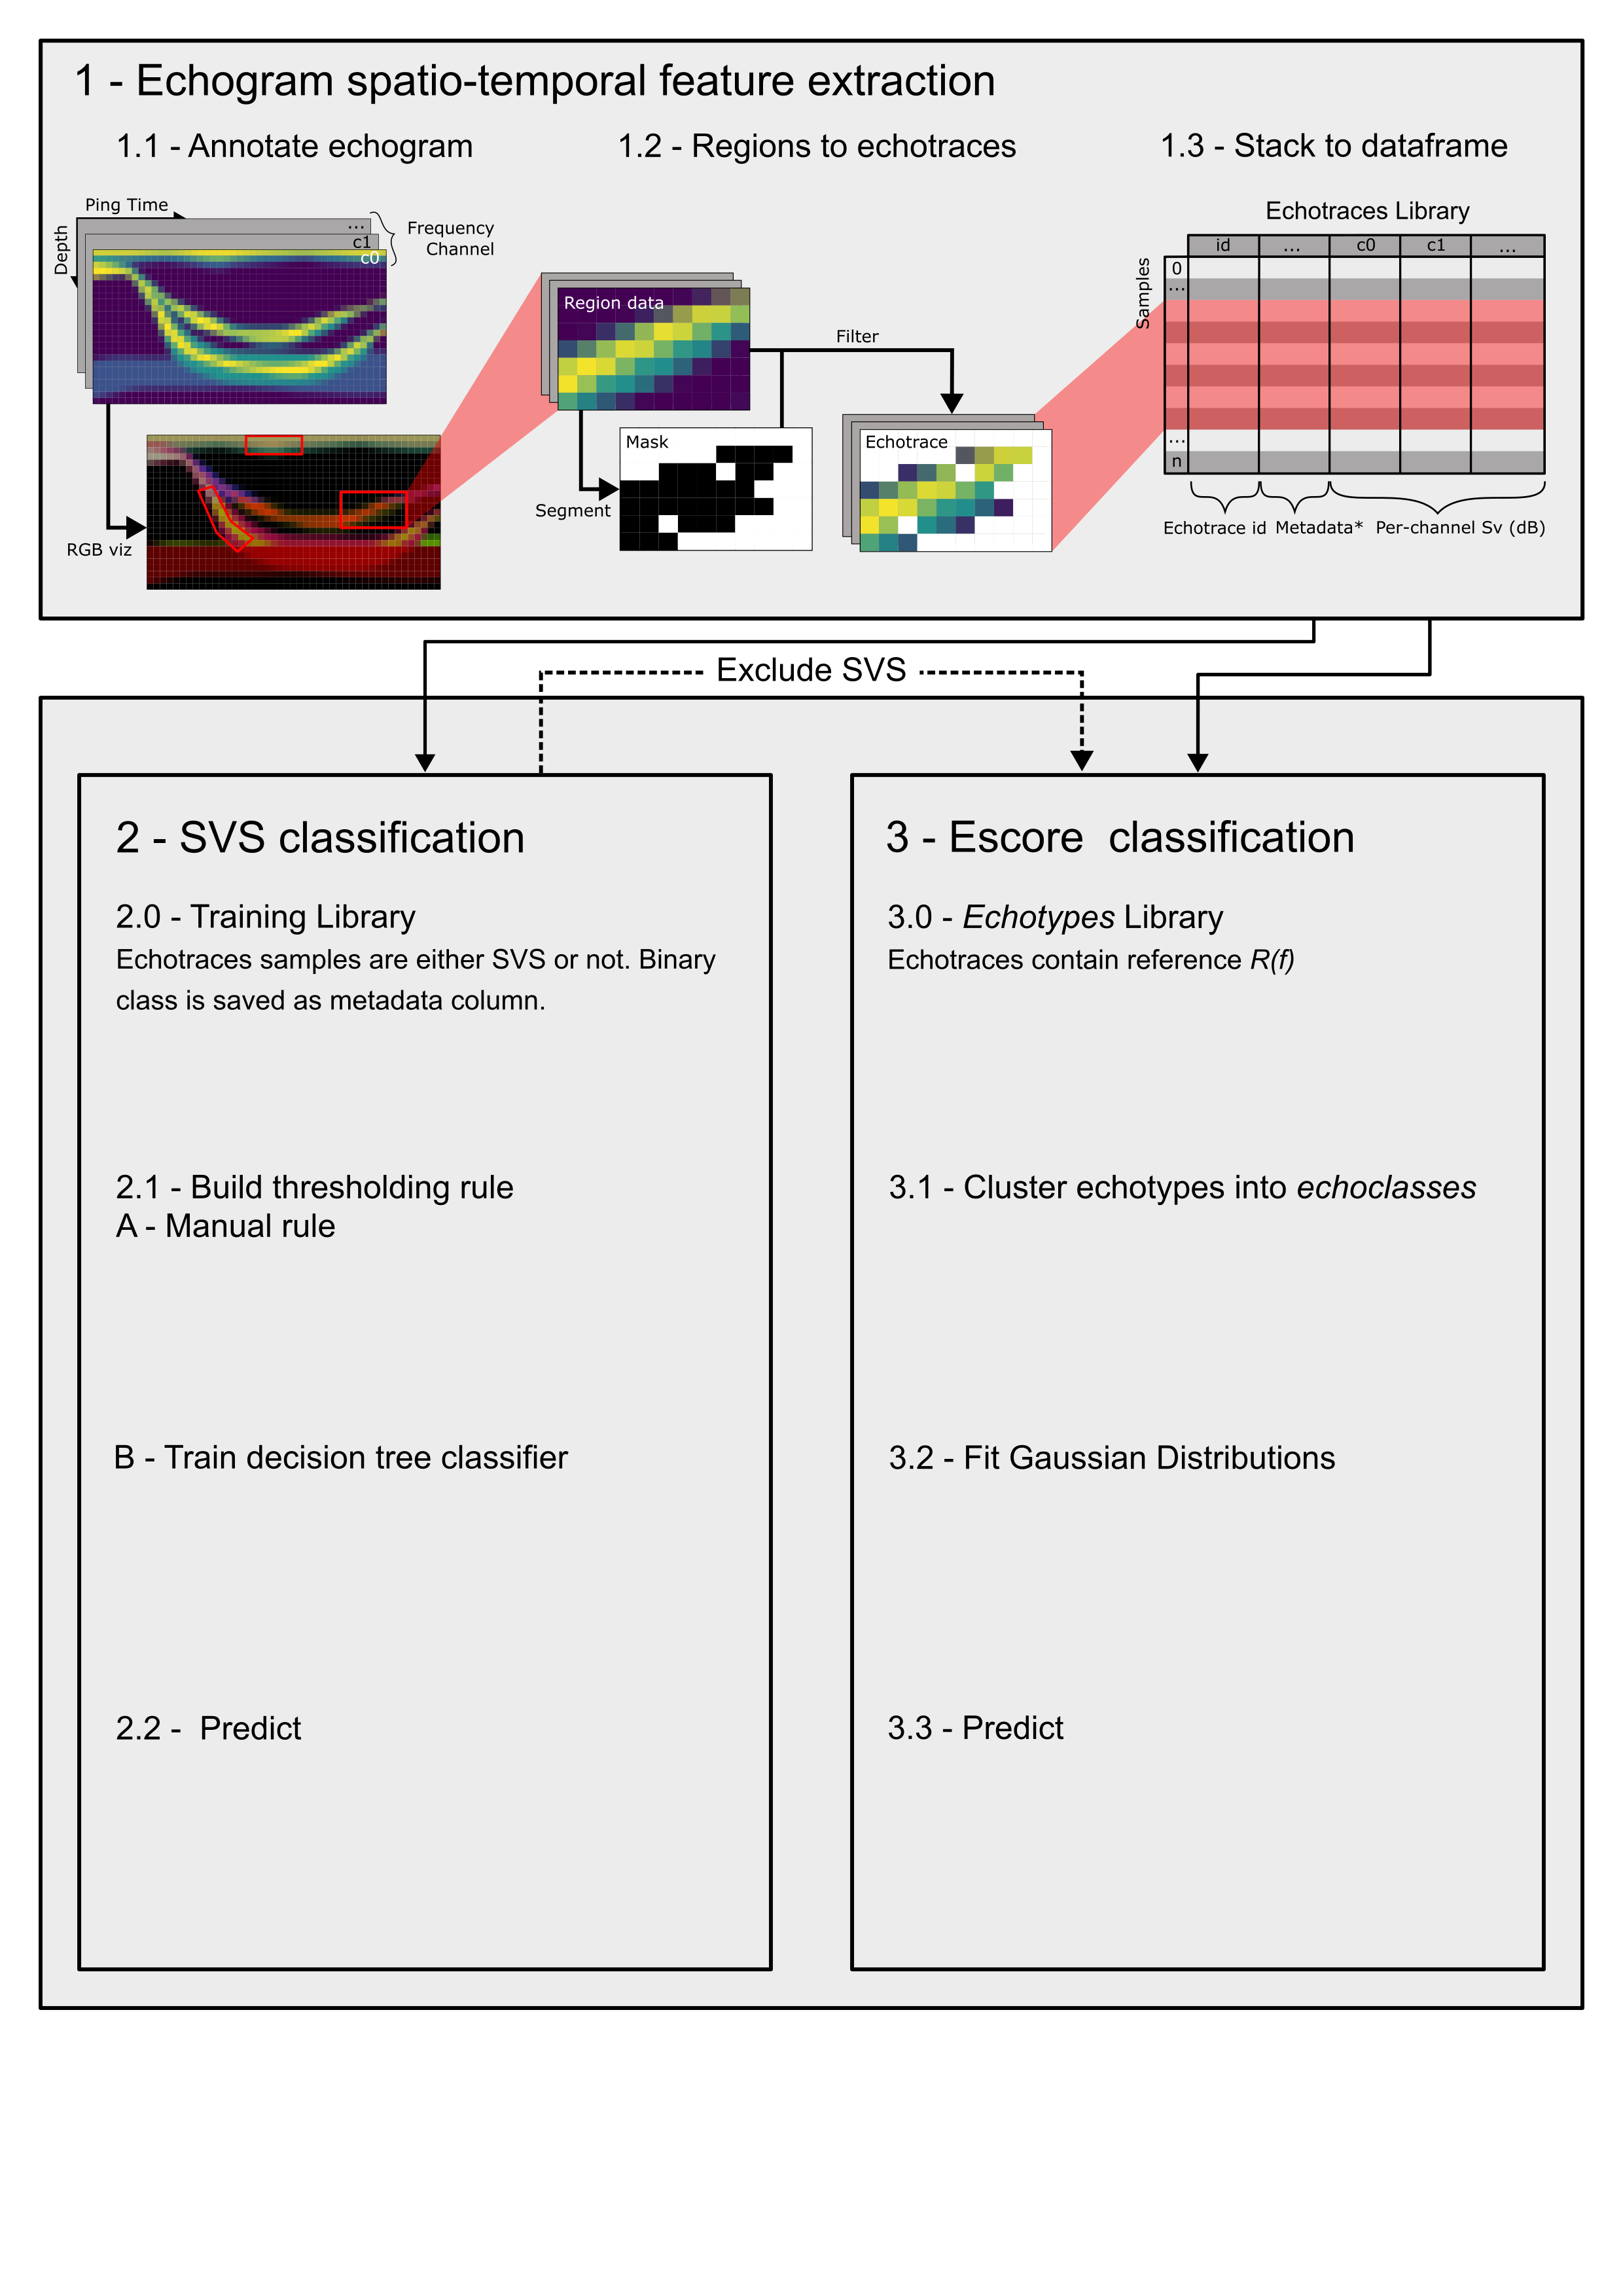
\includegraphics[width=1\linewidth,height=\textheight,keepaspectratio]{images/summary-fig.png}
\end{center}

\subsection{Data}\label{data}

Two oceanographic surveys, ABRAÇOS I and ABRAÇOS II, were performed in
the Southwest tropical Atlantic in Austral spring 2015 (September
29-October 21) and fall 2017 (April 9-March 8), as part of the project
`Acoustics along the Brazilian coast'
\citep{bertrand2015, bertrand2017}. The study area encompassed the
continental shelf and slope off Northeast Brazil, and oceanic waters
around the islands and seamounts of the Fernando de Noronha Chain.

Acoustic transects were conducted perpendicularly over the continental
slope, and radially around the Rocas Atoll and the Fernando de Noronha
Archipelago 1. Acoustic data were collected with a SIMRAD EK60
echosounder at 38, 70, 120 and 200 kHz, synchronously transmitting every
2-3 s. Volume backscattering strength `Sv' (dB re 1 m-1)
\citep{maclennan2002} was recorded down to 700 m depth with a pulse
duration of 512 \(\mu s\), beam angle of 7°, and a transmit power of
1000, 750 and 200 W at 38, 70 and 120 kHz, respectively. Standard target
calibration of the echosounder was conducted prior to data acquisition
\citep{demer2015}.

\subsection{Notebook 1 - Extracting fish-like echoes: the SVS
algorithm}\label{sec-svs-example}

\subsection{Notebook 2 - Mapping echo-classes
distribution}\label{notebook-2---mapping-echo-classes-distribution}

\begin{longtable}[]{@{}clccll@{}}
\caption[]{Typology of echogram features near the Fernando de Noronha
archipelago. *Time of day is relative to the observed diel vertical
migration and encoded as D (daytime), N (nighttime) and M (migration at
dawn or dusk).}\label{tbl-typology}\tabularnewline
\toprule\noalign{}
Code & Description & Daytime* & Frequency & ROIs & Echotypes \\
\midrule\noalign{}
\endfirsthead
\toprule\noalign{}
Code & Description & Daytime* & Frequency & ROIs & Echotypes \\
\midrule\noalign{}
\endhead
\bottomrule\noalign{}
\endlastfoot
Red1 & Fine epipelagic (20 - 100 m) layer with dominant 38 kHz response.
Less marked frequency response during night. Shaped with frequent upward
spikes, or as slender sublayer. & D, N, M & ++ & 26 & 26 \\
Green1 & Fine epipelagic layer with dominant 70 kHz response. Often
located below Red1. Hardly visible during night. & D, N, M & ++ & 20 &
18 \\
Blue1 & Small patches with dominant 120 kHz response, appearing pale
blue. Suspected crustacean hunting aggregations. & ? & - & 9 & 8 \\
Blue2 & Large layers with overall weak response dominated by the 120 kHz
channel, appearing dark blue. Seems only visible when no other acoustic
feature is present. Suspected crustacean layer. Underlying organisms
could be ubiquitous, although masked most of the time. Caution needed to
avoid selecting gain noise near acquisition range limit. & D, M & + & 13
& 6 \\
Fish1 & Dispersed structures with flat frequency response, visible below
and over the top layer formed by Red1 and Green1 during nighttime. Most
probably swim bladder-bearing fish. & D & ++ & 7 & 6 \\
Fish2 & Well defined layer aggregations mostly during migration or at
night. Flat frequency response, with localized shift toward 38 kHz,
potentially associated to tilt angle (selected ROIs containing either
frequency response). Believed to be swim bladder-bearing fish. & D, N, M
& ++ & 6 & 6 \\
Red2 & Weak layer occurring below Green1 or around 200 m during daytime.
38 kHz dominated. & D, M & + & 11 & 11 \\
Beige1 & Mesopelagic layer sometimes visible during day. 38 kHz
dominated but appear brownish or beige due to a weak 70 kHz response.
Possible mix involving Red2. & D & * & 4 & 4 \\
DeepGreen & & & & 2 & 2 \\
\end{longtable}

The Escore method is performed on samples contained within a 60 nm
radius from the Fernando de Noronha atoll.

The Escore method is performed on the ABRAÇOS II dataset only because of
significant seasonal variations in the acoustic seascapes
\citep{ariza2022}. Indeed, some level of homogeneity is required to
allow the model to account for changes in the dominant echo-classes with
space and time. Conversely, day-time and night-time are simultaneously
processed in spite of large differences. This is because some
echo-classes (\emph{e.g.} crustaceans-dominated) are only visible at
day-time, and masked at night due to a weak acoustic response. On the
other hand, some other are out of range during the day. Finally, while
migrations might appear to solve the issue, change in the mean tilt
angle of organism makes them poorly suited to be the only reference for
frequency response.\footnote{Should be interesting to perform Escore
  separately for each fPCA seascape. Maybe for the example, just in
  ABRAÇOS II pelagic + separate dawn, day, dusk, night. This can be done
  very easily after ROI selection. It also increases the chances of
  having a clustered structure in \(\Delta \text{MVBS}\) space.}

The 200 kHz channel is not used in the analysis because of its limited
depth range (180 m), constraining classification to the epipelagic zone.

The SVS rule induced in Section~\ref{sec-svs-example} is applied to the
dataset, and detected SVS are masked out prior to Escore analysis.

188 ROIs have been selected accross the whole echogram, either at day-
or night-time. Criteria for ROI selection were related to the frequency
responde homegeneity and relevance of the features within. While the
latter is highly subjective, peculiar attention was paid to frequently
observed features (\emph{e.g.} day-time scattering layer) or,
conversely, to potentially rare but well-defined aggregations
(\emph{e.g.} 120 kHz-dominated ``patches'' known to be associated to
crustaceans).

Selected ROIs, are processed using the \texttt{ExtractionWorkflow}. 160
(85 \%) are converted into echo-types while 28 are rejected.

\textbf{Extraction notes}

Extraction of echotypes with flat frequency responses tend to be
difficult when clustering \(\Delta \text{MVBS}\), probably because of a
large distribution of the features: the ROIs are contained in an
homegeneous seascape, and clustering just separates signals that are
already similar. In such cases (typically for Fish1 and Fish2) we apply
a clustering on \(\text{MVBS}\) directly, basically dropping the low
intensity samples. (also applies to some Red2).

Some extraction are better done by changing the reference frequency in
\(\Delta \text{MVBS}\) computation (e.g.~to 70 kHz for Green1 by day)

One Green1 actually a Fish1 (around beginning/middle) One Red1 actually
a Green1 (around end)

For Blue1: sometimes use thresholding on 120 kHz
(e.g.~\(\text{MVBS}_{120} \geq -67 \ \text{to} -72 \ \text{dB}\))

For Blue2: sometimes quite indulgent on the extraction criteria: no real
structure to see + distribution is hardly normal. But relative frequency
response is very strong in 120 kHz, with inter-freq variations
\textgreater\textgreater{} variances.

\begin{center}\rule{0.5\linewidth}{0.5pt}\end{center}

Frist seamount: new classes. Green surface: algae Maybe take more blues
Take some more: \textgreater{} 10 per user class

Test: remove seamounts 3D curtain plot of classif

\section{Development practices}\label{development-practices}

\begin{itemize}
\tightlist
\item
  Open-source (GitHub\ldots)
\item
  Modular design ()
\item
  Interoperability and integration in the scientific Python ecosystem
  (Data compatibility, Echoregions)
\item
  Reproducibility
\end{itemize}

Echolabel relies on Echoregions
(\url{https://github.com/echostack-org/echoregions}) to represent and
parse polygonal echogram annotations. Echoregions is an interfacing
package designed to represent acoustic data shapes annotations in Python
and easily plug into machine learning (ML) pipelines. It is part of the
Echostack suite \citep{lee2024}. While still in development, it presents
some key features which motivated using it to handle Echolabel's
annotations input-output, among which parsing and saving annotations in
EchoView's EVR file formats in addition to CSV files. This feature
enables Echolabel's output files to be converted to EVR format easily.
Further development of Echoregions should extend compatibility to other
echogram annotation formats \citep{lee2024}.

Another functionality is converting annotations to machine learning
ready masks (annotation to ML) and generating annotation from ML
predictions (ML to annotation). Annotation to ML is the primary use case
of Echolabel.

\section{Future directions}\label{future-directions}

\section{Conclusion}\label{conclusion}

\subsection*{References}\label{references}
\addcontentsline{toc}{subsection}{References}

\renewcommand{\bibsection}{}
\bibliography{references.bib}


\nolinenumbers


\end{document}
